\documentclass[11pt]{beamer}
\usetheme{metropolis}

\usepackage[utf8]{inputenc}
\usepackage[spanish]{babel}
\usepackage[T1]{fontenc}

\usepackage{amsmath}
\usepackage{amsfonts}
\usepackage{amssymb}
\usepackage{graphicx}
\usepackage{url}
\usepackage{booktabs}
%\usepackage{emoji}

\DeclareMathOperator{\sen}{sen}
\DeclareMathOperator{\tg}{tg}

\setbeamertemplate{caption}[numbered]


\title[C**dre Overleaf]{Trascendiendo \textit{Overleaf}}
\subtitle{Escribiendo papers colaborativos con \texttt{git} + \LaTeX\ + LLMs opensource}
\author[Barriga]{Diego Barriga\\
	\texttt{dbarriga@ciencias.unam.mx}
}
\institute[UNAM]{
	Optica-UNAM Student Chapter, Facultad de Ciencias\\
	Universidad Nacional Autónoma de México
}
\date{16 de Mayo 2026}
\titlegraphic{
    \begin{minipage}{\textwidth}
        \raggedright
        
\includegraphics[width=1cm]{img/logo_unam_negro.jpg}
        \hfill
    \end{minipage}
}
\setbeamertemplate{navigation symbols}{}

%\newcommand{\email}{email}

\bibliographystyle{apalike}

% La agenda se mostrará al inicio de cada sección
\AtBeginSection[]
{
	\begin{frame}
		\frametitle{Contenido}
		\tableofcontents[currentsection]
	\end{frame}
}

\begin{document}

\begin{frame}
	\titlepage
\end{frame}

\begin{frame}{Contenido}
\tableofcontents
\end{frame}

\begin{frame}
	\begin{figure}
		\centering
		
\includegraphics[width=0.55\textwidth]{img/trap.jpg}
		\caption{It's a trap!!!}
	\end{figure}
\end{frame}

\begin{frame}{Disclaimer I}
	\LARGE En este taller \textbf{no} aprenderás \LaTeX\
\end{frame}

\begin{frame}{Disclaimer II}
\LARGE Aquí aprenderas a usar \texttt{git} para crear \alert{trabajos colaborativos} en \LaTeX\ con un \textit{twist} de límon\footnote{LLMs locales}
\end{frame}

\section{Motivaciones}

\begin{frame}{¿Porqué migrar \textit{Overleaf} $\rightarrow$ \texttt{git}?}
	\begin{itemize}
		\item <1-> Tiempo de compilación ilimitado\footnote{Dependerá de la tostadora que uses como compu}
		\item <2-> No tienes que pagar para trabajo colaborativo\footnote{No tienes que compartir tu cuenta}
		\item <3-> Lo anterior es mentira, si pagaste por tu compu. Usala \texttt{:-)}
		\item <5-> Control de versiones de tus documentos grado industrial
		\item <6-> Puedes usar LLM locales y de pago como asistentes de escritura
	\end{itemize}
\end{frame}

\begin{frame}
\Large Estas herramientas son \textbf{alternativas} a tu flujo de trabajo actual no una sustitución.
\end{frame}

\begin{frame}[fragile]{Check check check}
	\begin{enumerate}
		\item Intalado software básico
		\begin{enumerate}
			\item \LaTeX
			\item \texttt{git}
			\item \texttt{ollama}
			\item Vs Code + extensiones
		\end{enumerate}
		\item Compilación de un archivo \texttt{*.tex}
		\item Configuración de \texttt{git}
	\end{enumerate}

	\begin{verbatim}
    git config --global user.name "Dieguito Maradona"
    git config --global user.email "me@barriga.mx"
    \end{verbatim}
\end{frame}

\section{Fundamentos de \texttt{git}}

\begin{frame}{¿Qué es \texttt{git} y pa' que sirve?}
	Software libre cuyo proposito es versionar los archivos de un \textbf{directorio de trabajo} dado. Se le conoce como \alert{sistema de control de versiones}.

	\begin{columns}
        \begin{column}{0.5\textwidth}
            \begin{figure}
                \centering
                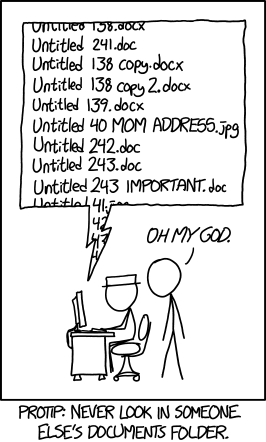
\includegraphics[width=0.55\textwidth]{img/xkcd_docs.png}
                \caption{\url{https://xkcd.com/1459/}}
            \end{figure}
        \end{column}

        % Second Column
        \begin{column}{0.5\textwidth}
            \begin{figure}
                \centering
                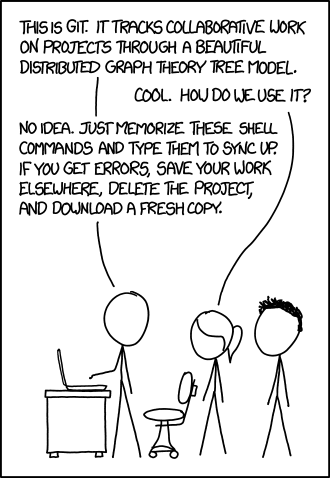
\includegraphics[width=0.65\textwidth]{img/git.png}
                \caption{\url{https://xkcd.com/1597/}}
            \end{figure}
        \end{column}
    \end{columns}
\end{frame}

\begin{frame}{Sistema de control de versiones}
	\begin{itemize}
		\item Guardado de versiones de archivos
		\item Visualizar diferencias entre archivos
		\item Trabaja con texto principalmente
		\item Asociación de cambios con autoræs
		\item Regresar en el tiempo a versiones anteriores
	\end{itemize}
\end{frame}

\begin{frame}{(Pre) Historia}
	\begin{itemize}
		\item Creado en el contexto del desarrollo del \href{https://www.youtube.com/watch?v=5iFnzr73XXk}{kernel de linux}
		\item Enfoque distribuido
		\item Velocidad y simpleza
		\item Creación de multiples ramas
		\item Varias desarrolladoras trabajando en un mismo proyecto 
	\end{itemize}
\end{frame}

\begin{frame}{Áreas de trabajo}

	\begin{enumerate}
		\item \textit{Working Directory}
		\item \textit{Staging Area}
		\item \textit{Local repository}
	\end{enumerate}
	\pause
	\begin{alertblock}{¿Cómo mover entre áreas?}
		    \begin{itemize}
        \item \texttt{git init} $\rightarrow$ Iniciar un repositorio en el directorio actual
        \item \texttt{vim archivo.c} $\rightarrow$ Modifica un archivo y git detecta cambios
        \item \texttt{git add} $\rightarrow$ Envía las modificaciones al \textit{staging area}
        \item \texttt{git commit} $\rightarrow$ Guarda los cambios del \textit{staging area} en el directorio \texttt{.git}
        \item \texttt{git restore} $\rightarrow$ Deshacer cambios en el \textit{staging area}
    \end{itemize}
	\end{alertblock}
\end{frame}

\begin{frame}
	\begin{figure}
		\centering
		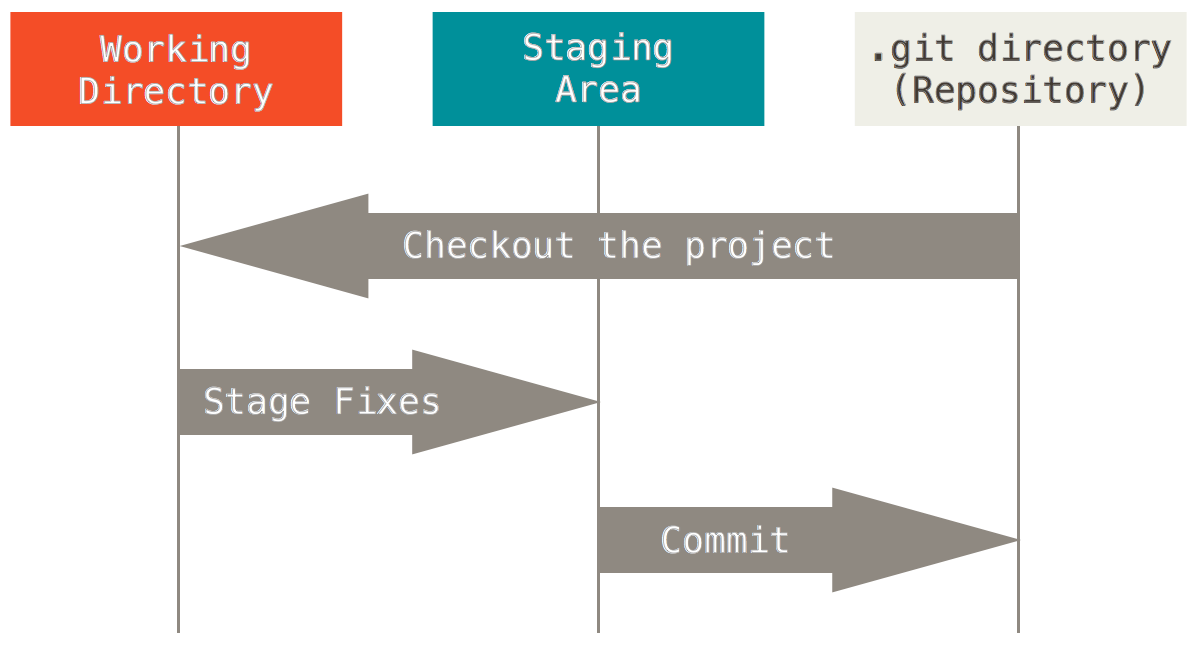
\includegraphics[width=\textwidth]{img/git_areas.png}
		\caption{Áreas de git}
	\end{figure}
\end{frame}

\section{Crash course \texttt{git}}

\begin{frame}{Respositorios}
	Hay dos tipos de repositorios. Locales y remotos.
	\begin{alertblock}{Comandos}
		\begin{itemize}
			\item Local $\rightarrow$ \texttt{\$ git init}
			\item Remoto $\rightarrow$ \texttt{\$ git clone <url>}
		\end{itemize}	
	\end{alertblock}
\end{frame}

\begin{frame}{Moviendo archivos entre áreas}

	\begin{alertblock}{Commandos}
		\begin{itemize}
			\item \texttt{\$ git add} $\rightarrow$ Mueve archivos al área de \alert{staging}\footnote{Esta área es previa a cambios definitivos (\alert{commit})}
			\begin{itemize}
				\item Agregar achivos individuales - \texttt{git add main.py}
				\item Agregar por extension - \texttt{git add *.cpp}
				\item Agregar todo en un directorio - \texttt{git add .}
			\end{itemize} 
			\item \texttt{\$ git commit} $\rightarrow$ Confirma los cambios que esten en el area de \alert{staging}. Se crea un punto en la historia del proyecto.
			\item \texttt{\$ git restore} $\rightarrow$ Devuelve el archivo al estado original del último \alert{commit}.
			\begin{itemize}
				\item Agregar mensaje de confirmación - \texttt{git commit -m ``Mensaje''}
			\end{itemize}
			\item \texttt{\$ git restore ---staged} $\rightarrow$ Descarta los cambios del área de \alert{staging}\footnote{Esto es, devolverlos al \alert{working directory}}.
		\end{itemize}
	\end{alertblock}
\end{frame}

\begin{frame}{Commit}
	Confirma los cambios que esten en el area de staging. Se crea un punto en la historia del proyecto
	\pause
	\begin{block}{Buenas prácticas}
		\begin{itemize}
			\item El commit debe ser acompañado con un mensaje descriptivo de los cambios
			\item Es mejor hacer varios commits que hagan una cosa pequeña en lugar de un solo commit con muchos cambios
			\item Recomendable seguir algun estandar. Ya sea definido por el equipo o algún otro\footnote{\url{https://www.freecodecamp.org/news/how-to-write-better-git-commit-messages/}}
		\end{itemize}		
	\end{block}
\end{frame}

\begin{frame}
	\begin{figure}
		\centering
		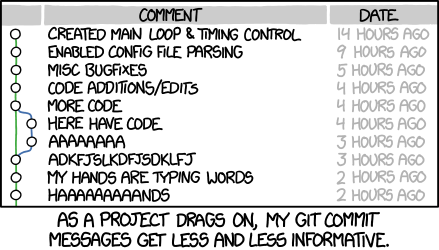
\includegraphics[width=\textwidth]{img/commits.png}
		\caption{https://xkcd.com/1296/}
	\end{figure}
\end{frame}

\begin{frame}{Comprobando el estado}

	Verificamos el estado actual del repositorio. ¿Qué cambios hubo y dónde?

	\begin{alertblock}{Commando}
		\begin{itemize}
			\item \texttt{\$ git status}
			\begin{itemize}
				\item \texttt{.gitignore} $\rightarrow$ Archivo de texto que permite excluir archivos y carpetas para que \texttt{git} los ignore.
			\end{itemize}
			\item \texttt{\$ git log} $\rightarrow$ Muestra el historial de \alert{commits}, sus mensajes y quien realizó los cambios.
			\item \texttt{\$ git diff} $\rightarrow$ Muestra los cambios en archivos
		\end{itemize}
	\end{alertblock}
\end{frame}

\begin{frame}{Ramas}
	\begin{figure}
		\centering
		
\includegraphics[width=0.5\textwidth]{img/branch_meme.jpg}
		\caption{Un meme sobre ramas de \texttt{git}}
	\end{figure}
\end{frame}

\begin{frame}{Killer function}
	\begin{itemize}
		\item Parte fundamental del software \texttt{git} es su manejo de ramas (o \alert{branches})
		\item Trabajar con ramas permite explorar nuevos desarrollos sin romper, ensuciar o arruinar nuestra rama principal
		\begin{itemize}
			\item Considerenlo un universo paralelo (o multiverso)
			\item Trabajar en diferentes versiones del software de forma simultanea
		\end{itemize}
	\end{itemize}
\end{frame}

\begin{frame}
	\begin{figure}
		\centering
		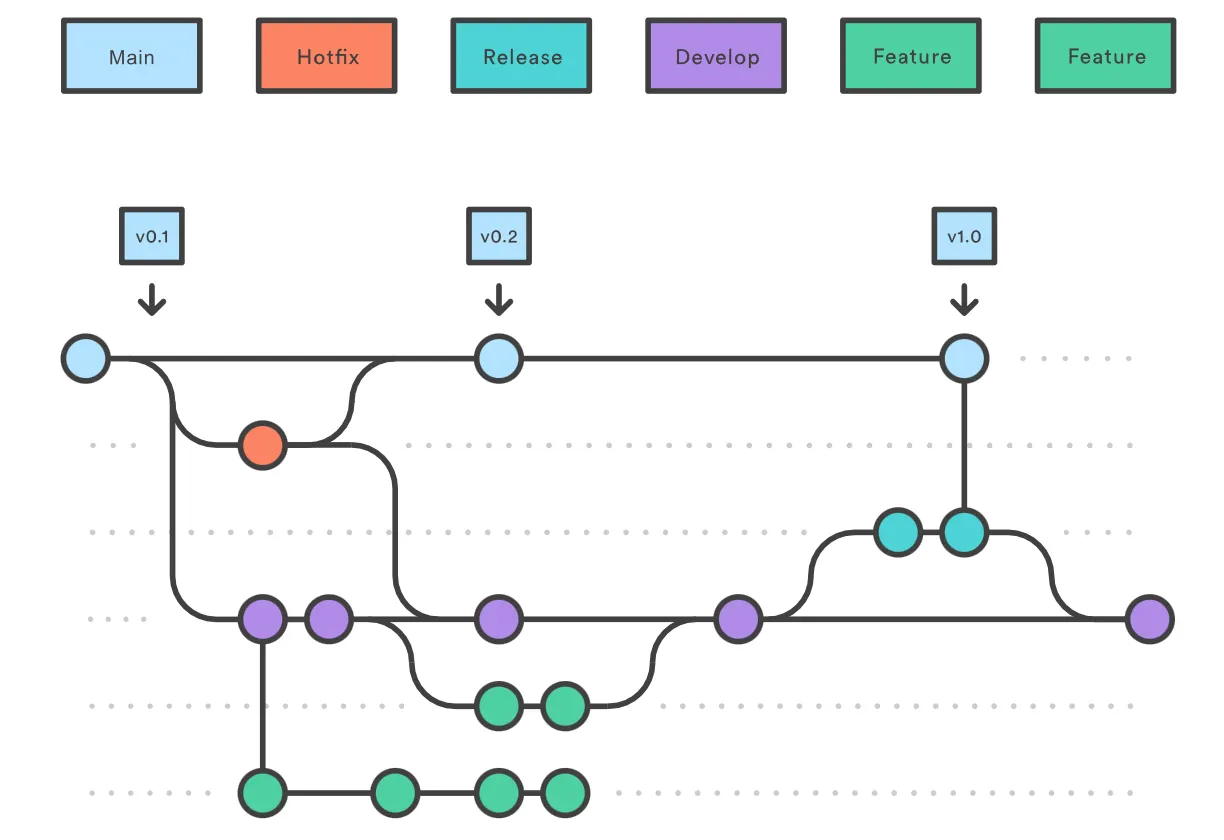
\includegraphics[width=\textwidth]{img/branches.png}
		\caption{Asi se ve una historia de \texttt{git}}
	\end{figure}	
\end{frame}

\begin{frame}
	\begin{alertblock}{Comandos para ramas}
		\begin{itemize}
			\item \texttt{\$ git switch [-c] <nueva-rama>} $\rightarrow$ Cambia a una nueva rama. Si se agrega la bandera \texttt{-c} crea la rama si no existe.
			\item \texttt{\$ git branch} $\rightarrow$ Muestra las ramas existentes.
			\item \texttt{\$ git merge} $\rightarrow$ Combina cambios de una rama a otra.
		\end{itemize}
	\end{alertblock}
\end{frame}

\begin{frame}{Repositorios remotos}
	\begin{itemize}
		\item Hasta ahora todos los cambios que hemos hecho han sucedido en localmente. 
		\item \texttt{git} permite trabajar con repositorios \alert{remotos}. Esto es, repositorios que se encuentran en otras computadoras.
	\end{itemize}
\end{frame}

\begin{frame}
	\begin{figure}
		\centering
		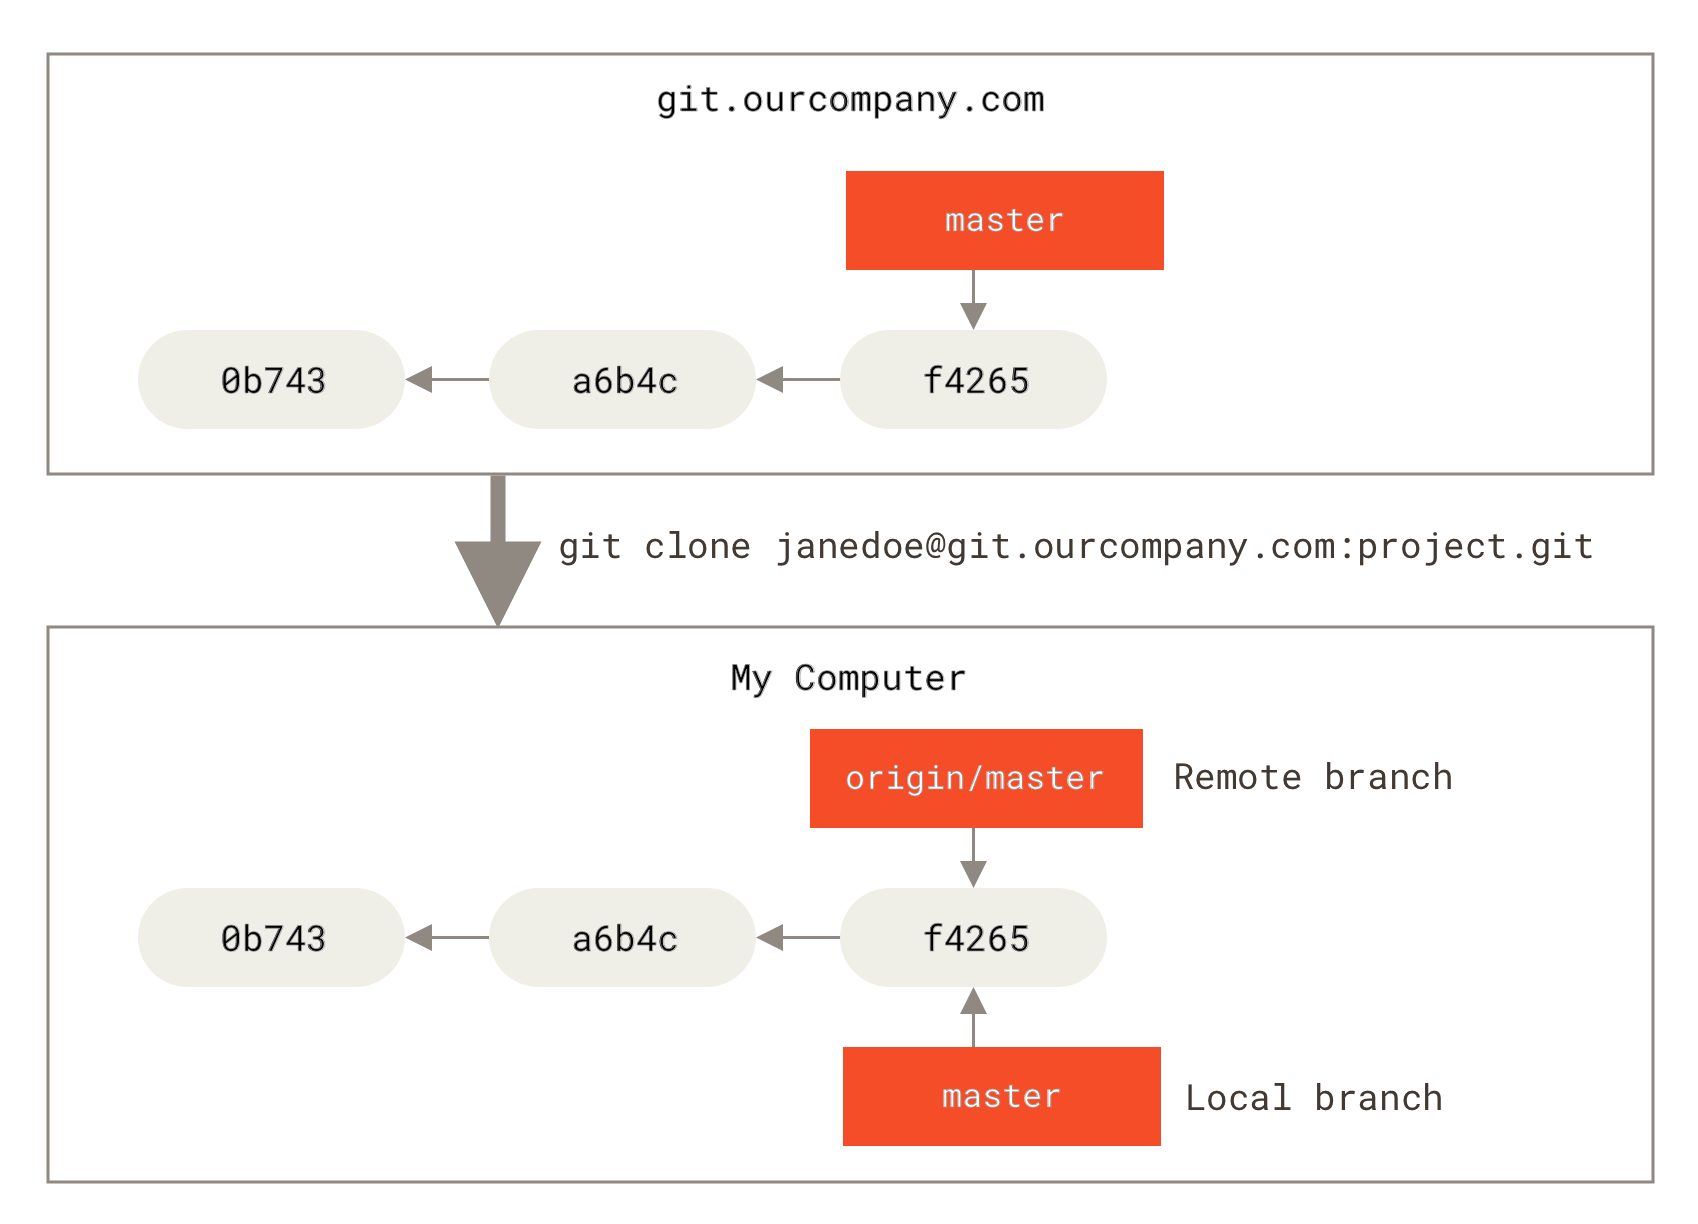
\includegraphics[width=\textwidth]{img/remote.png}
	\end{figure}
\end{frame}

\begin{frame}
	\begin{alertblock}{Comandos}
		\begin{itemize}
			\item \texttt{\$ git remote -v} $\rightarrow$ Muestra los repositorios remotos configurados.
			\item \texttt{\$ git remote add <nombre-remoto> <url>} $\rightarrow$ Agrega un repositorio remoto.
			\item \texttt{\$ git push <nombre-remoto> <rama>} $\rightarrow$ Sube los cambios locales al repositorio remoto.
			\item \texttt{\$ git pull <nombre-remoto> <rama>} $\rightarrow$ Descarga los cambios del repositorio remoto.
		\end{itemize}
	\end{alertblock}
\end{frame}

\section{Trabajo colaborativo}

\begin{frame}{Plataformas de alojamiento}
	\begin{columns}[t] % [t] aligns columns at the top
        % First Row
        \begin{column}{0.5\textwidth}
            \begin{figure}
                \centering
                
\includegraphics[width=0.6\textwidth]{img/github_logo.png} \\
                \small \url{https://github.com}
            \end{figure}
        \end{column}
        \begin{column}{0.5\textwidth}
            \begin{figure}
                \centering
                
\includegraphics[width=0.6\textwidth]{img/gitlab_logo.png}	
                \small \url{https://gitlab.com}
            \end{figure}
        \end{column}
    \end{columns}

    \vspace{0.5cm} % Adds vertical space between rows

    \begin{columns}[t]
        % Second Row
        \begin{column}{0.5\textwidth}
            \begin{figure}
                \centering
                
\includegraphics[width=0.7\textwidth]{img/gittea_logo.png} \\
                \small \url{https://about.gitea.com/}
            \end{figure}
        \end{column}
        \begin{column}{0.5\textwidth}
            \begin{figure}
                \centering
                
\includegraphics[width=0.5\textwidth]{img/codeberg_logo.png} \\
                \small \url{https://codeberg.org}
            \end{figure}
        \end{column}
    \end{columns}
\end{frame}

\begin{frame}{Forks}
	\begin{itemize}
		\item Un fork es una copia de un respositorio remoto pero que ahora es de tu autoría.
		\item El respositorio original queda \textbf{ligado} con la copia que realizaste.
		\item Por medio de forks es que podemos realizar \alert{contribuciones} a respositorios ajenos.
	\end{itemize}
	\begin{alertblock}{Comando}
		\begin{itemize}
			\item \texttt{\$ git clone <url>}
		\end{itemize}
	\end{alertblock}
\end{frame}

\begin{frame}
	\begin{figure}
		\centering
		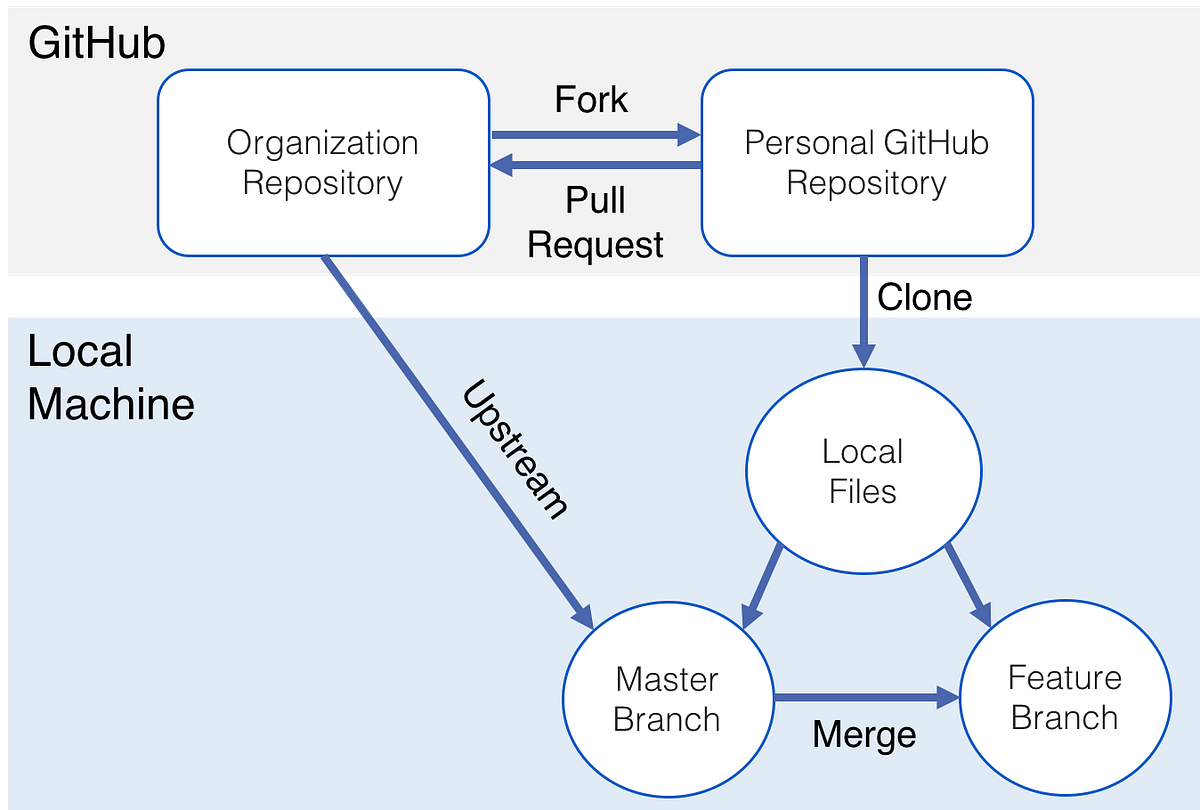
\includegraphics[width=\linewidth]{img/fork.png}
		\caption{Diagrama de un fork}
	\end{figure}
\end{frame}

\begin{frame}{Personal Access Token (PAT)}
	Este token nos permitirá comunicarnos con el alojamiento remoto sin necesidad de usar nuestra contraseña real\footnote{GitHub ya no soporta utilizar la contraseña real por seguridad}.

	\begin{exampleblock}{Pasos para GitHub}
		\begin{enumerate}
			\item \textbf{Configuración:} Ve a \textit{Settings} $\rightarrow$ \textit{Developer settings}.
			\item \textbf{Generación:} Selecciona \textit{Personal access tokens} $\rightarrow$ \textit{Tokens (classic)}.
			\item \textbf{Permisos:} Haz clic en \textit{Generate new token} y selecciona los permisos necesarios (mínimo: \texttt{repo}).
			\item \textbf{Guardado:} Copia el token inmediatamente. \textbf{No podrás verlo de nuevo.}
		\end{enumerate}
	\end{exampleblock}
\end{frame}

\begin{frame}
	
	\Large El token es una credencial privada. \alert{Nunca} lo compartas. Si se filtra, revócalo inmediatamente desde la web.
    
\end{frame}

\begin{frame}{Pull request (PR)}
	
	Un PR es una solicitud para fusionar cambios de una rama de algun \alert{fork} a otra (generalmente la rama principal o \texttt{main}).
    
	\pause

	\begin{exampleblock}{Beneficios}
		\begin{itemize}
			\item \textbf{Revisión de cambios:} Otros colaboradores pueden comentar y sugerir cambios.
			\item \textbf{Discusión:} Permite rebotar ideas y tener una discusión sobre los cambios.
			\item \textbf{Historial:} Deja un registro de \textbf{por qué} se hizo un cambio específico.
    	\end{itemize}
	\end{exampleblock}
    
	\pause
    \begin{exampleblock}{Flujo Típico}
        \texttt{Push branch} $\rightarrow$ \texttt{Abrir PR} $\rightarrow$ \texttt{Revisión/Aprobación} $\rightarrow$ \texttt{Merge}
    \end{exampleblock}
\end{frame}

\begin{frame}
	\begin{figure}
		\centering
		
\includegraphics[width=0.7\textwidth]{img/pr_meme.png}
		\caption{\url{https://www.monkeyuser.com/2018/pull-request/}}
	\end{figure}
\end{frame}

\begin{frame}{Buenas Prácticas de Pull Requests}
    \begin{itemize}
        \item \textbf{Mantenlo simple:} PRs pequeños y enfocados en una sola tarea (más fáciles de revisar).
        \item \textbf{Descripciones Claras:} Explicar el \textit{qué} y el \textit{por qué} del cambio.
        \item \textbf{Auto-revisión:} Revisar tus cambios antes de solicitar la revisión de otros.
        \item \textbf{Feedback Constructivo:} Comentarios enfocados en los cambios, no en la persona.
    \end{itemize}
    \pause
    \begin{alertblock}{Regla de Oro}
        Nunca hagas \textit{merge} de un PR sin que haya sido revisado por al menos una persona más.
    \end{alertblock}
\end{frame}

\begin{frame}{Ejemplo academico}
	\begin{figure}
		\centering
		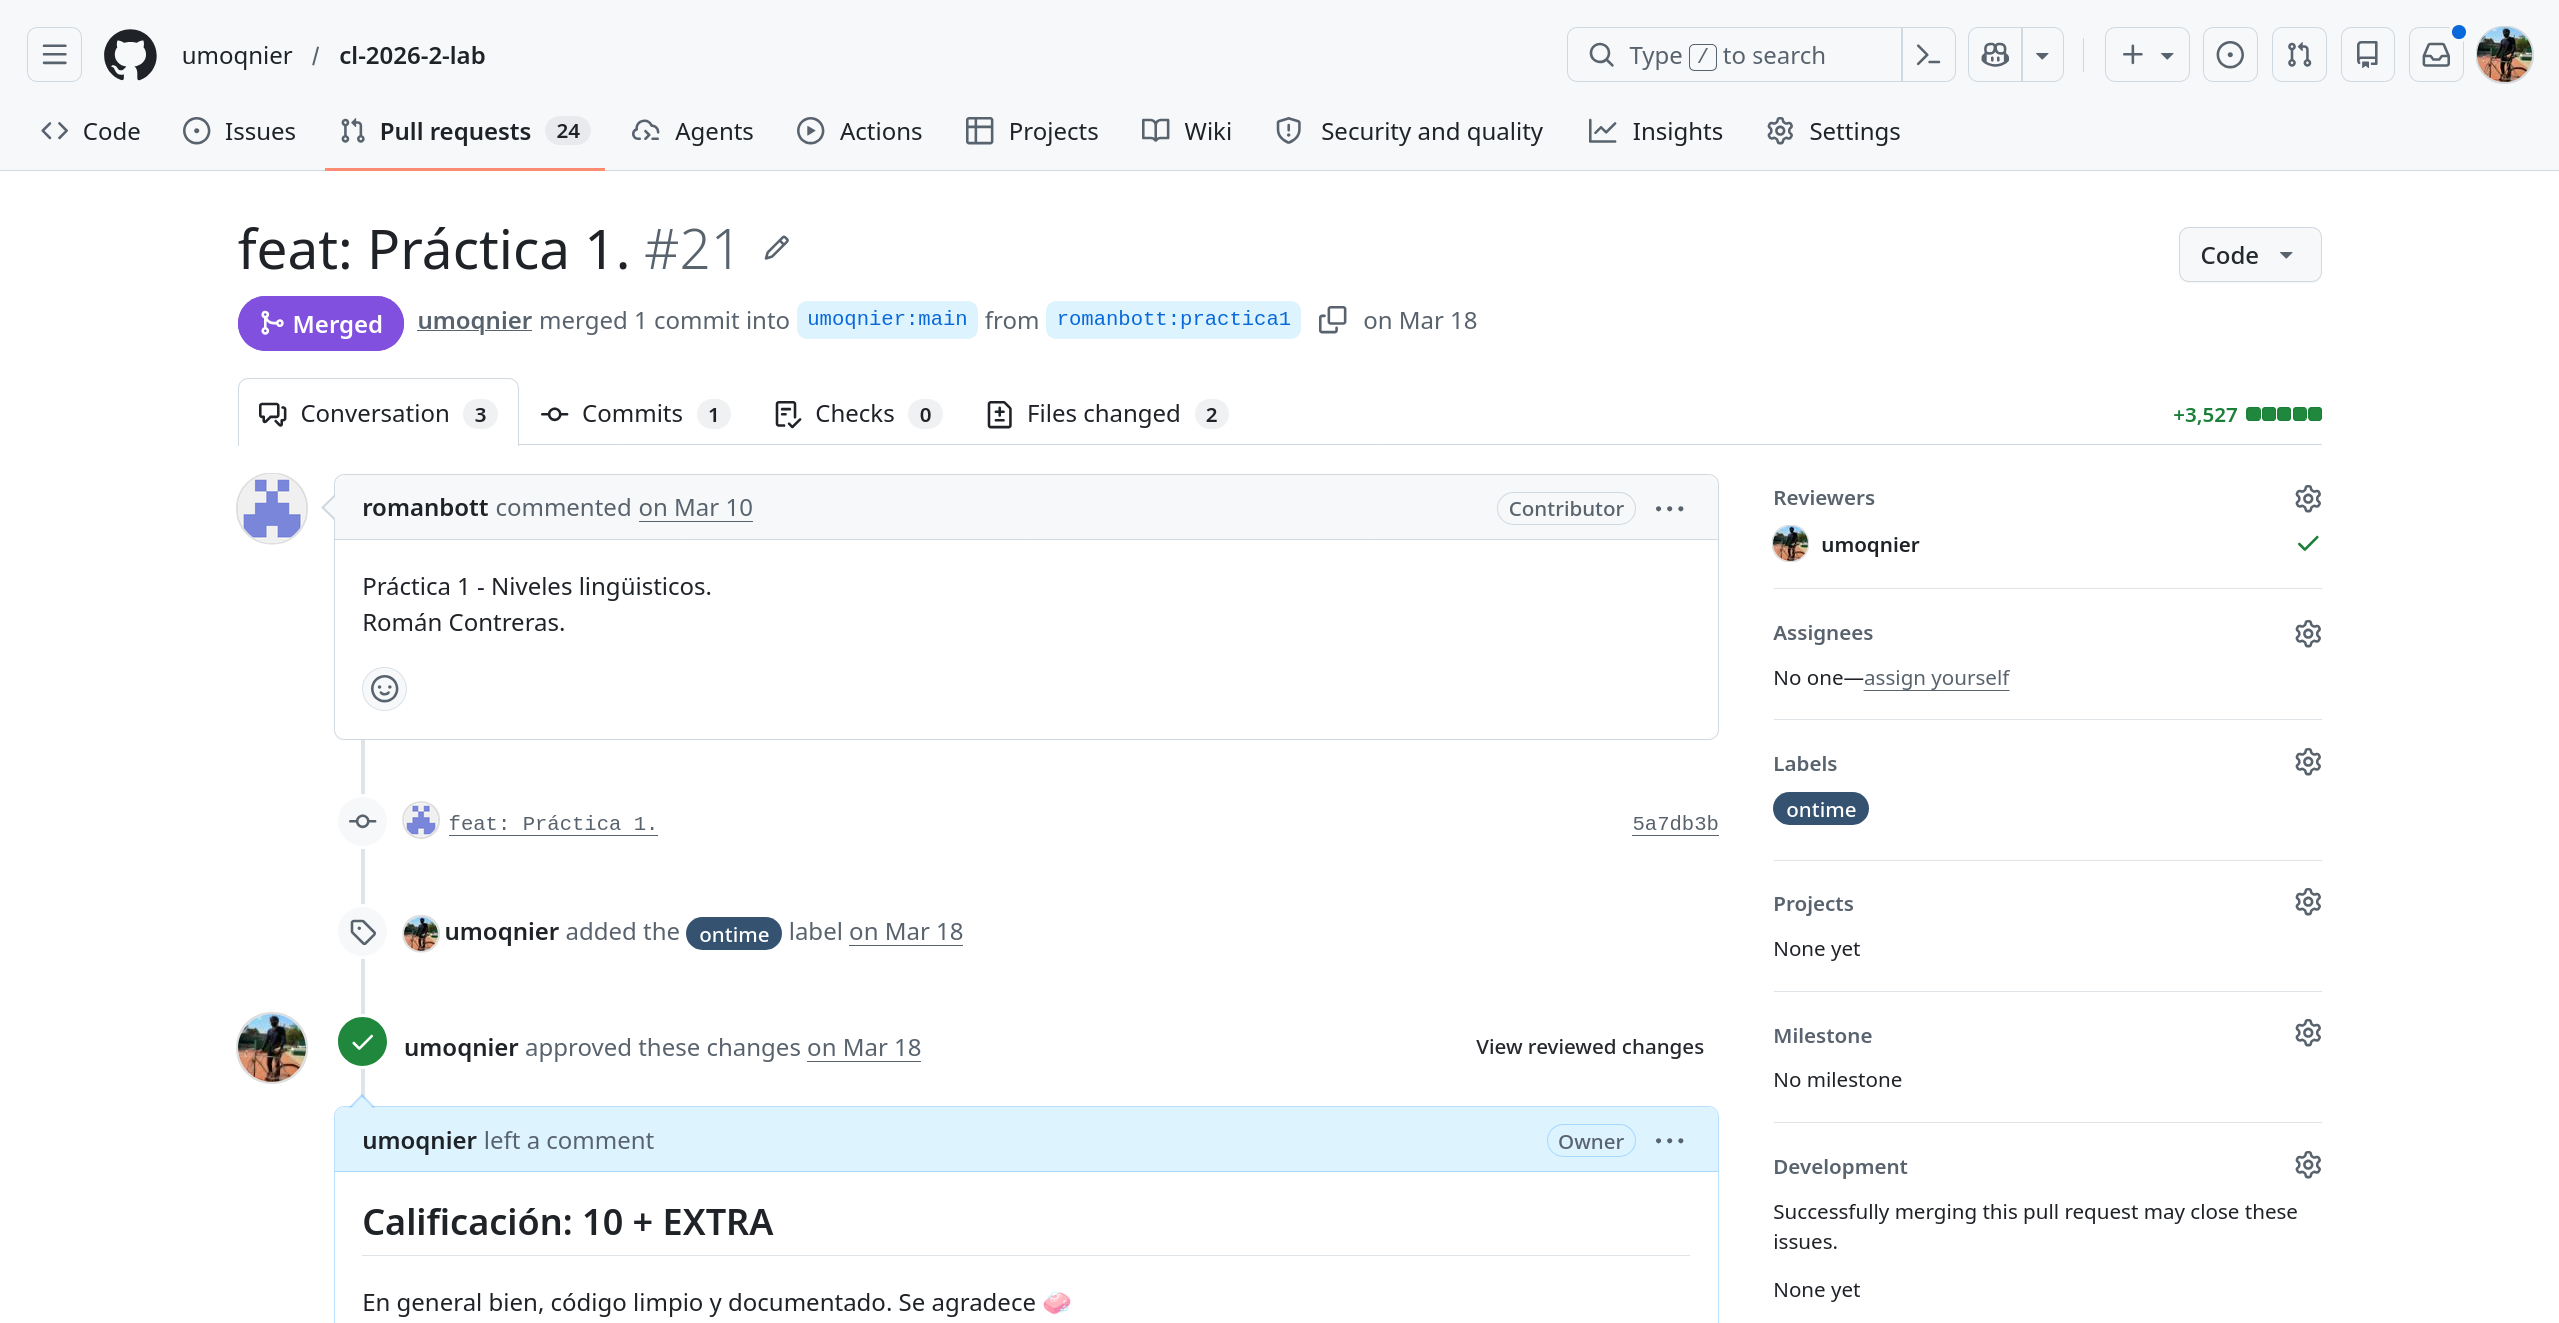
\includegraphics[width=\textwidth]{img/pr_clase.png}
		\caption{\url{https://github.com/umoqnier/cl-2026-2-lab/pull/21}}
	\end{figure}
\end{frame}

\begin{frame}{Ejemplo desarrollo software libre}
	\begin{figure}
		\centering
		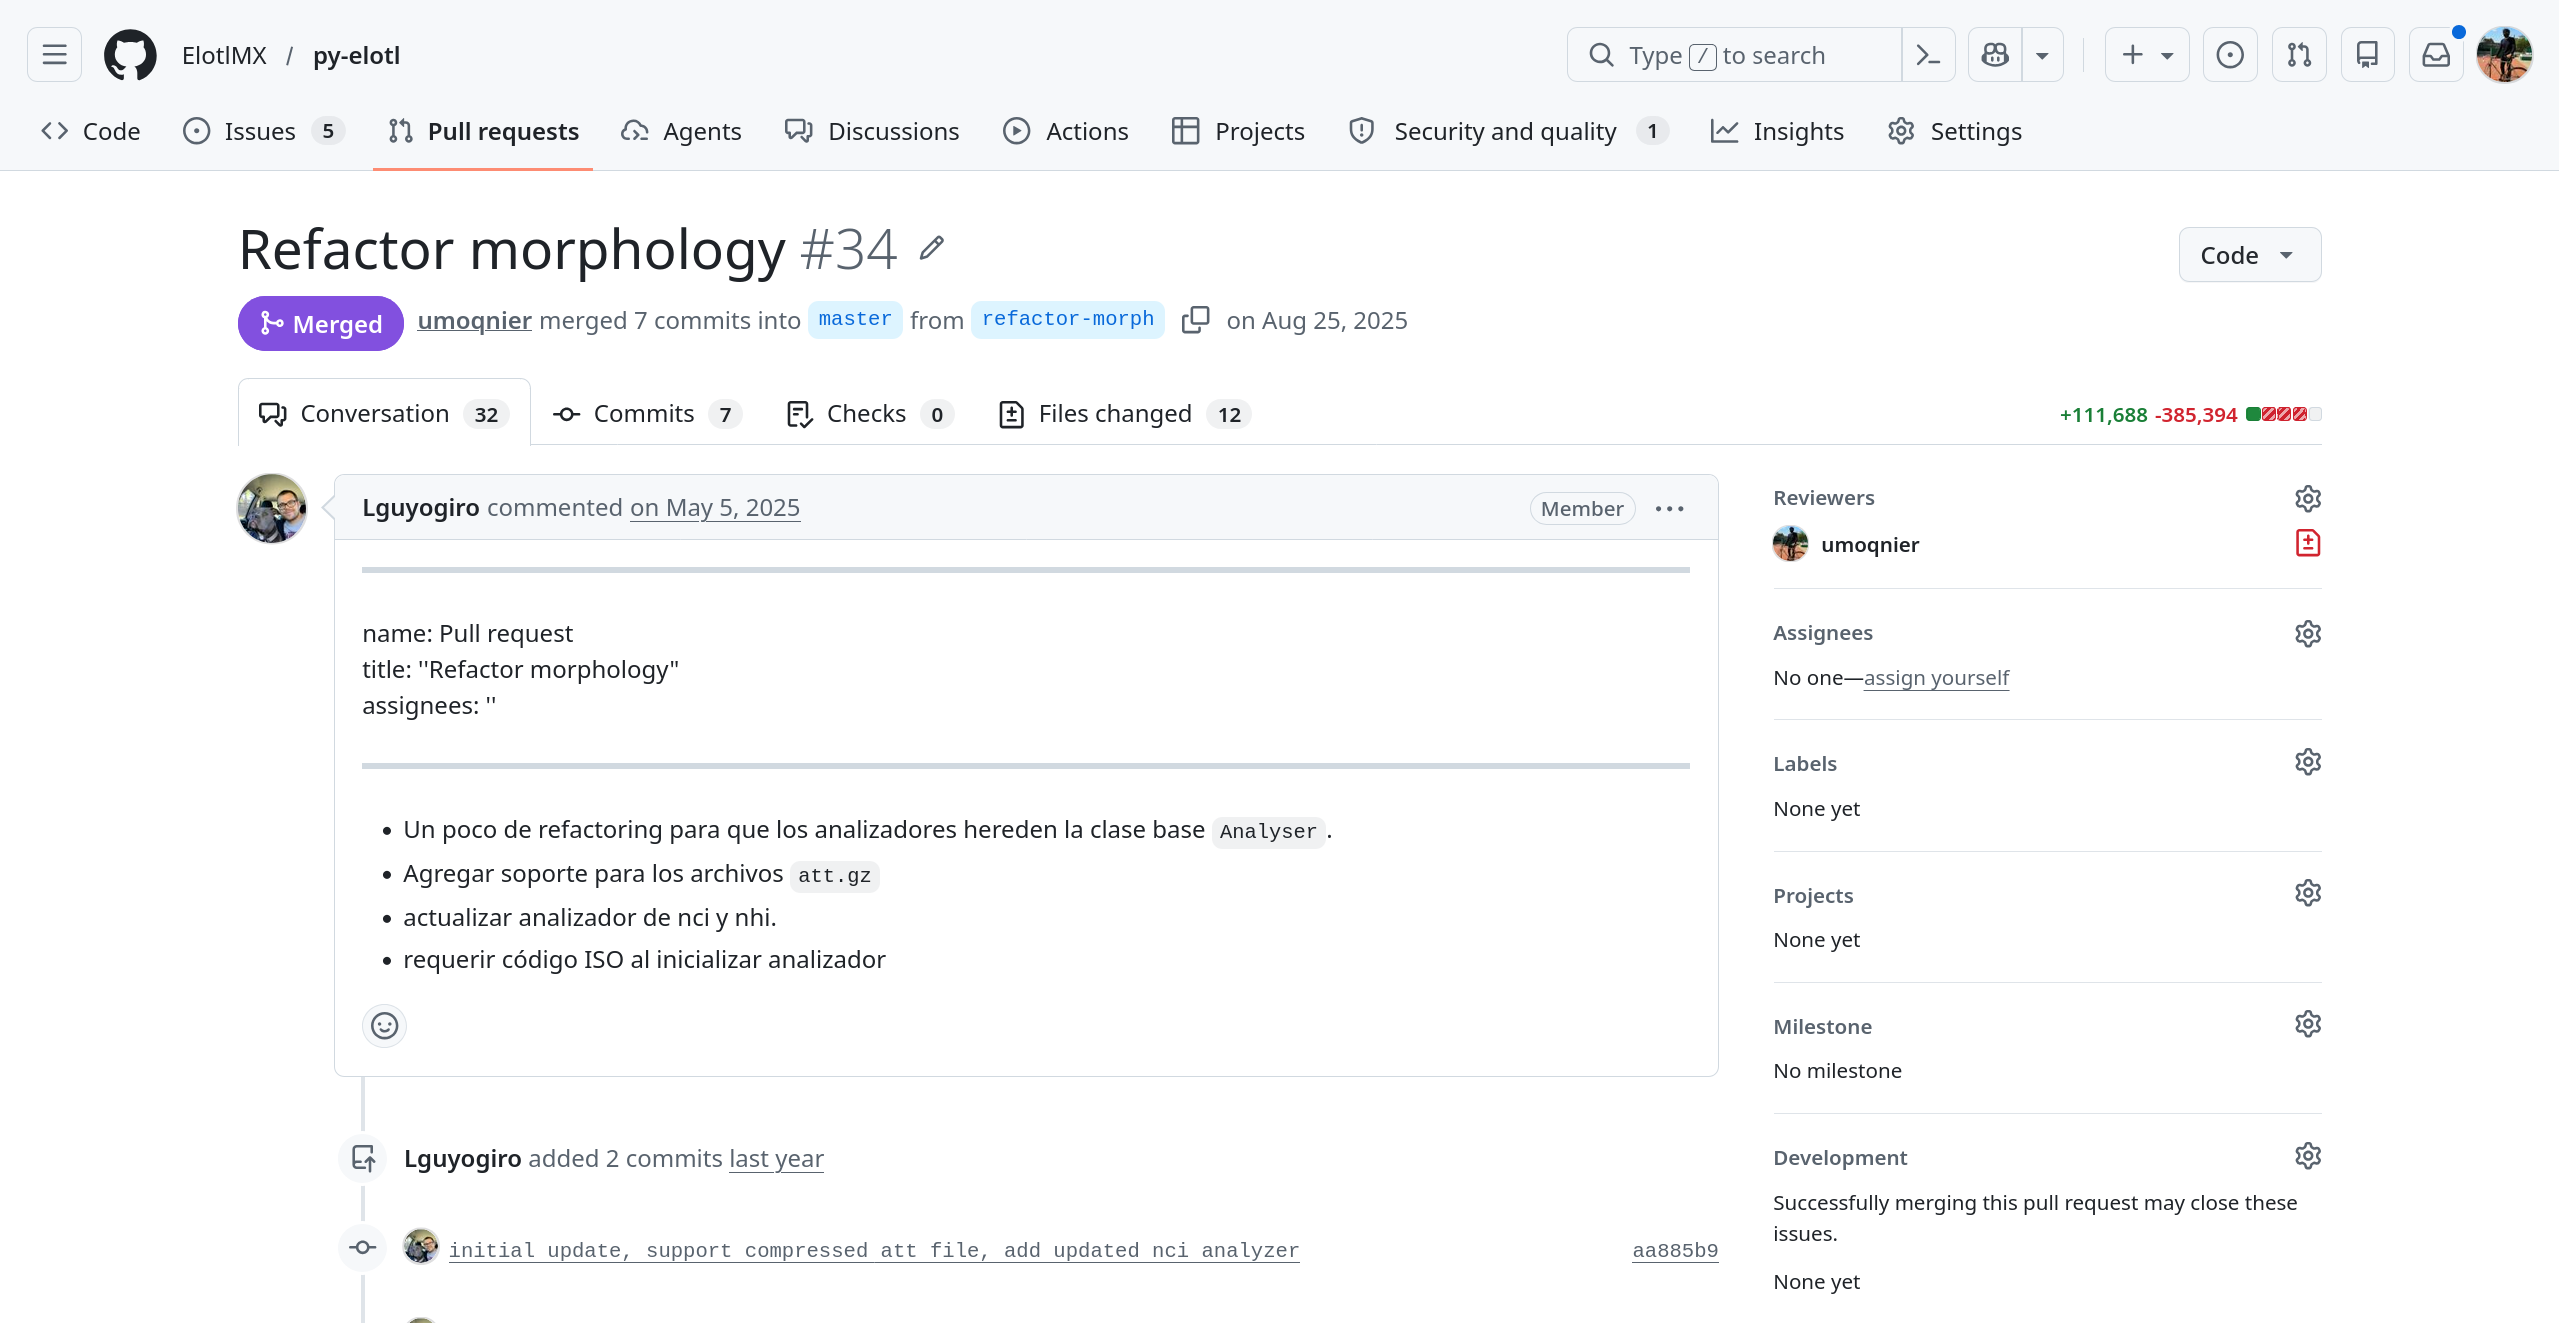
\includegraphics[width=\textwidth]{img/pr_elotl.png}
		\caption{\url{https://github.com/ElotlMX/py-elotl/pull/34}}
	\end{figure}
\end{frame}

\begin{frame}{Resolución de conflictos}
	 
     Un \alert{conflicto}\footnote{Un conflicto no es un error del sistema, es una solicitud de intervención humana para evitar la pérdida de datos.} ocurre cuando dos personas (o dos ramas) modifican la \textbf{misma línea} del \textbf{mismo archivo}, y Git no puede decidir automáticamente cuál versión mantener.
\end{frame}

\begin{frame}{Flujo de resolución}
    \begin{enumerate}
        \item \textbf{Detección:} Git detiene el \texttt{merge} y marca los archivos en conflicto.
        \item \textbf{Edición:} Abres el archivo y buscas las \textit{marcas de conflicto}.
        \item \textbf{Decisión:} Eliges conservar tu cambio, el cambio entrante, o ambos.
        \item \textbf{Finalización:} Guardas el archivo, haces \texttt{git add} y \texttt{git commit}.
    \end{enumerate}
\end{frame}

\section{Desarrollo latex local}

\section{Modelos del lenguaje locales (o casi)}

\begin{frame}{Herramientas}
	
\end{frame}

\begin{frame}{Config basica}
	
\end{frame}



\begin{frame}[allowframebreaks]{Referencias}
	\small
    %\bibliographystyle{plain}
    %\bibliography{bibliografia}
\end{frame}

\end{document}